% !TEX TS-program = pdflatexmk
\documentclass[12pt]{article}

% Layout.
\usepackage[top=1in, bottom=0.75in, left=1in, right=1in, headheight=1in, headsep=6pt]{geometry}

% Fonts.
\usepackage{mathptmx}
\usepackage[scaled=0.86]{helvet}
\renewcommand{\emph}[1]{\textsf{\textbf{#1}}}
\newcommand{\ans}[1][1in]{\rule{#1}{.5pt}}

\usepackage[parfill]{parskip}

% Misc packages.
\usepackage{amsmath,amssymb,latexsym}
\usepackage{graphicx,hyperref}
\usepackage{array}
\usepackage{xcolor}
\usepackage{multicol,tikz}
\usepackage{tabularx,colortbl,booktabs,xparse}
\usepackage{enumitem}

\newcommand{\be}{\begin{enumerate}}
\newcommand{\ee}{\end{enumerate}}

% Rotation: \rot[<angle>][<width>]{<stuff>}
\NewDocumentCommand{\rot}{O{45} O{1em} m}{\makebox[#2][l]{\rotatebox{#1}{#3}}}%

\usepackage{fancyhdr}
\pagestyle{fancy} 
\lhead{\large\sf\textbf{MATH F113X: Introduction to Hamiltonian Circuits and Paths}}
%\chead{\large\sf\textbf{lecture notes}}
%\rhead{\large\sf\textbf{Day 1}}

\begin{document}

\emph{Terminology:} Hamiltonian Path, Hamiltonian Circuit
\begin{enumerate}


\item A \emph{Hamiltonian circuit} (sometimes called Hamiltonian Cycle) is

\vfill

\item A \emph{Hamiltonian path} is

\vfill

\item Some Example Graphs\\
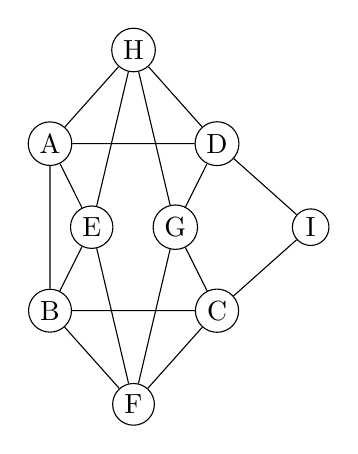
\begin{tikzpicture}[scale=1.5]
\tikzstyle{every node}=[circle, draw, fill=white,
                        inner sep=2pt]
\node (1) at (-0.707, 0.707){A};
\node (2) at (-0.707, -0.707){B};
\node (3) at (0.707, -0.707){C};
\node (4) at (0.707, 0.707){D};
\node (5) at (-0.354, 0.){E};
\node (6) at (0., -1.5){F};
\node (7) at (0.354, 0.){G};
\node (8) at (0., 1.5){H};
\node (9) at (1.5,0){I};
\foreach \i/\j in {1/2,1/4,1/5,1/8,2/3,2/5,2/6,9/3,9/4,3/6,3/7,4/7,4/8,5/6,5/8,6/7,7/8}{\draw (\i) -- (\j);}
\end{tikzpicture}
\hfill
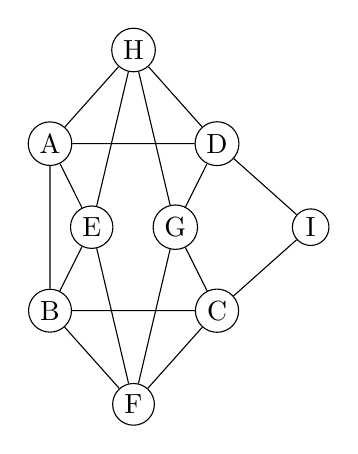
\begin{tikzpicture}[scale=1.5]
\tikzstyle{every node}=[circle, draw, fill=white,
                        inner sep=2pt]
\node (1) at (-0.707, 0.707){A};
\node (2) at (-0.707, -0.707){B};
\node (3) at (0.707, -0.707){C};
\node (4) at (0.707, 0.707){D};
\node (5) at (-0.354, 0.){E};
\node (6) at (0., -1.5){F};
\node (7) at (0.354, 0.){G};
\node (8) at (0., 1.5){H};
\node (9) at (1.5,0){I};
\foreach \i/\j in {1/2,1/4,1/5,1/8,2/3,2/5,2/6,9/3,9/4,3/6,3/7,4/7,4/8,5/6,5/8,6/7,7/8}{\draw (\i) -- (\j);}
\end{tikzpicture}
\hfill
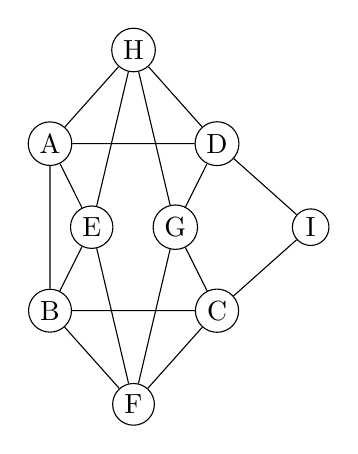
\begin{tikzpicture}[scale=1.5]
\tikzstyle{every node}=[circle, draw, fill=white,
                        inner sep=2pt]
\node (1) at (-0.707, 0.707){A};
\node (2) at (-0.707, -0.707){B};
\node (3) at (0.707, -0.707){C};
\node (4) at (0.707, 0.707){D};
\node (5) at (-0.354, 0.){E};
\node (6) at (0., -1.5){F};
\node (7) at (0.354, 0.){G};
\node (8) at (0., 1.5){H};
\node (9) at (1.5,0){I};
\foreach \i/\j in {1/2,1/4,1/5,1/8,2/3,2/5,2/6,9/3,9/4,3/6,3/7,4/7,4/8,5/6,5/8,6/7,7/8}{\draw (\i) -- (\j);}
\end{tikzpicture}

\vfill

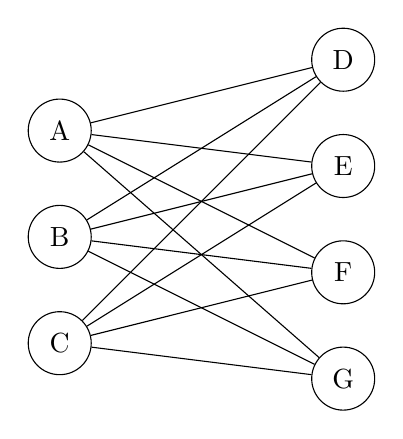
\begin{tikzpicture}[scale=0.9, every node/.style={circle, draw, minimum size=8mm}]
% Left partition (3 nodes)
\node (A) at (0, 3) {A};
\node (B) at (0, 1.5) {B};
\node (C) at (0, 0) {C};
% Right partition (4 nodes)
\node (D) at (4, 4) {D};
\node (E) at (4, 2.5) {E};
\node (F) at (4, 1) {F};
\node (G) at (4, -0.5) {G};
% All edges
\foreach \u in {A, B, C}
    \foreach \v in {D, E, F, G}
        \draw (\u) -- (\v);
\end{tikzpicture}
\hfill
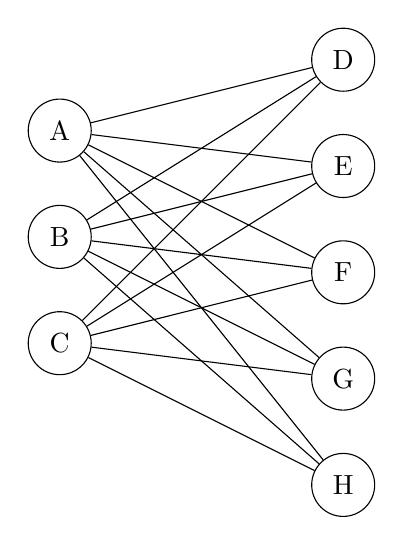
\begin{tikzpicture}[scale=0.9, every node/.style={circle, draw, minimum size=8mm}]
% Left partition (3 nodes)
\node (A) at (0, 3) {A};
\node (B) at (0, 1.5) {B};
\node (C) at (0, 0) {C};
% Right partition (4 nodes)
\node (D) at (4, 4) {D};
\node (E) at (4, 2.5) {E};
\node (F) at (4, 1) {F};
\node (G) at (4, -0.5) {G};
\node (H) at (4, -2) {H};
% All edges
\foreach \u in {A, B, C}
    \foreach \v in {D, E, F, G, H}
        \draw (\u) -- (\v);
\end{tikzpicture}
\hfill
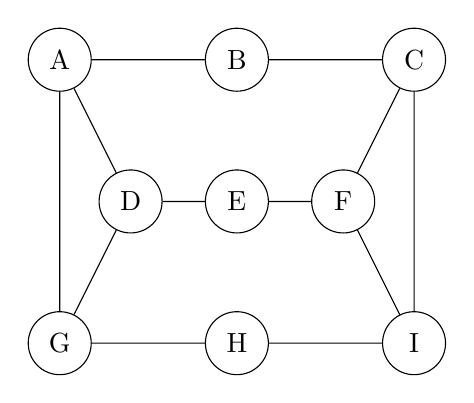
\begin{tikzpicture}[scale=0.9, every node/.style={circle, draw, minimum size=8mm}]
\node (A) at (-.5,4) {A};
\node (B) at (2,4) {B};
\node (C) at (4.5,4) {C};
\node (D) at (0.5,2) {D};
\node (E) at (2,2) {E};
\node (F) at (3.5, 2) {F};
\node (G) at (-.5,0) {G};
\node (H) at (2,0) {H};
\node (I) at (4.5,0) {I};
\draw (G) -- (A) -- (B) -- (C) -- (F) -- (E) -- (D) -- (G) -- (H) --(I) --(C) (A)--(D)(F)--(I);
\end{tikzpicture}

\vfill
\item Do any of the above graphs have an \textbf{Euler} circuit?
\newpage
\item What would a Hamiltonian circuit in the graph below represent?\\

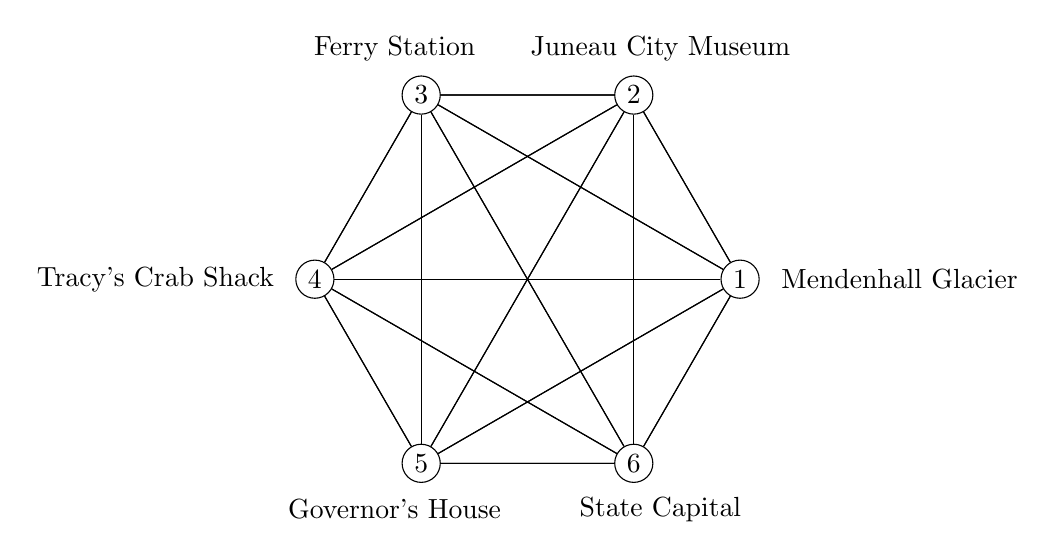
\begin{tikzpicture}[scale=1.35]
\node at (0:3.5){Mendenhall Glacier};
\node at (60: 2.5){Juneau City Museum};
\node at (120: 2.5){Ferry Station};
\node at (180: 3.5){Tracy's Crab Shack};
\node at (240: 2.5){Governor's House};
\node at (300: 2.5){State Capital};
\tikzstyle{every node}=[circle, draw, fill=white,
                        inner sep=2pt]
\node (1) at (0:2){1};
\node (2) at (60:2){2};
\node (3) at (120:2){3};
\node (4) at (180:2){4};
\node (5) at (240:2){5};
\node (6) at (300:2){6};
\foreach \i in {1,2,...,6}{
	\foreach \j in {1,2,...,6}{
		\draw (\i) -- (\j);
		}
		}
\end{tikzpicture}
\vfill


\item Why might you want to find a Hamiltonian circuit of smallest weight? How might you do that?

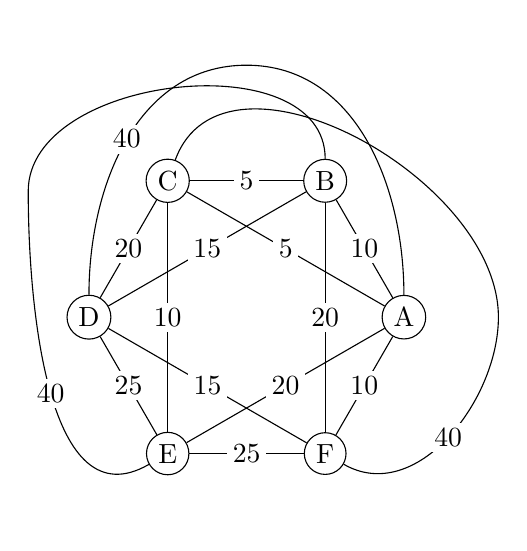
\begin{tikzpicture}[scale=1,lbl/.style={inner sep = 2pt, fill = white}]
\tikzstyle{vtx}=[circle, draw, inner sep=2pt]
\node[vtx] (1) at (0:2){A};
\node[vtx]  (2) at (60:2){B};
\node[vtx]  (3) at (120:2){C};
\node[vtx]  (4) at (180:2){D};
\node[vtx]  (5) at (240:2){E};
\node[vtx]  (6) at (300:2){F};
% phantom coordinates outside the circle for the three diameter edges
\coordinate (AD) at (90:3.2);   % A is at 0°, D at 180°, midpoint points up
\coordinate (BE) at (150:3.2);  % B is at 60°, E at 240°, midpoint points down-left
\coordinate (CF) at (0:3.2);  % C is at 120°, F at 300°, midpoint points down-right
\foreach \i/\j/\k in {1/2/10,1/3/5,1/5/20,1/6/10,2/4/15,2/6/20,2/3/5,3/4/20,4/5/25,5/6/25,3/5/10,4/6/15}{\draw (\i) --node[lbl]{\k} (\j);}
\draw (1) to[out=90,in=0]   (AD) to[out=180,in=90]  node[lbl]{40} (4);
\draw (2) to[out=90,in=90] (BE) to[out=270,in=210] node[lbl]{40} (5);
\draw (3) to[out=70,in=90](CF) to[out=270,in=330]  node[lbl]{40} (6);
\end{tikzpicture}
\hfill
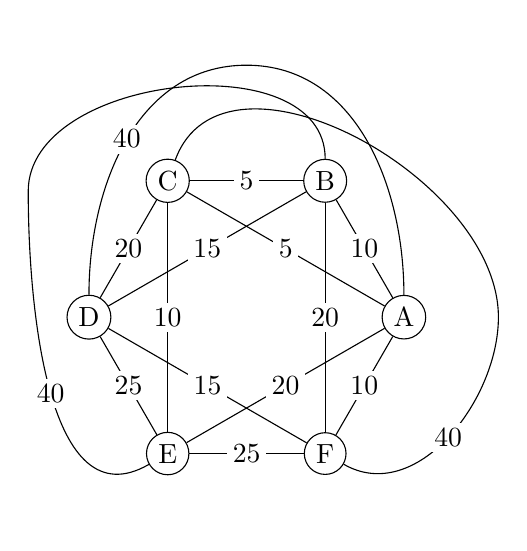
\begin{tikzpicture}[scale=1,lbl/.style={inner sep = 2pt, fill = white}]
\tikzstyle{vtx}=[circle, draw, inner sep=2pt]
\node[vtx] (1) at (0:2){A};
\node[vtx]  (2) at (60:2){B};
\node[vtx]  (3) at (120:2){C};
\node[vtx]  (4) at (180:2){D};
\node[vtx]  (5) at (240:2){E};
\node[vtx]  (6) at (300:2){F};
% phantom coordinates outside the circle for the three diameter edges
\coordinate (AD) at (90:3.2);   % A is at 0°, D at 180°, midpoint points up
\coordinate (BE) at (150:3.2);  % B is at 60°, E at 240°, midpoint points down-left
\coordinate (CF) at (0:3.2);  % C is at 120°, F at 300°, midpoint points down-right
\foreach \i/\j/\k in {1/2/10,1/3/5,1/5/20,1/6/10,2/4/15,2/6/20,2/3/5,3/4/20,4/5/25,5/6/25,3/5/10,4/6/15}{\draw (\i) --node[lbl]{\k} (\j);}
\draw (1) to[out=90,in=0]   (AD) to[out=180,in=90]  node[lbl]{40} (4);
\draw (2) to[out=90,in=90] (BE) to[out=270,in=210] node[lbl]{40} (5);
\draw (3) to[out=70,in=90](CF) to[out=270,in=330]  node[lbl]{40} (6);
\end{tikzpicture}

\vfill

\vfill
\item Comments on a concrete application and counting.
\vfill

\vfill
\end{enumerate}
\end{document}
